% !TEX root = ../notes.tex

lets\marginnote{\emph{Lecture 3}}[0mm] try and formalise some of these ideas. So consider,
$$ \di N t = f(N) $$
where $N \in \R, t \in \R, f : \R \to \R$. Then we define steady states as, where $f(N^*) = 0$. These are also reffered to as fixed points or equilibrium. When a system in the first place depends on whether the state is attracting.
\begin{ndefi}[Attrracting]
  A steady state $N^*$ is attracting if all trajectories that start close to $N^*$ approach it as $t \to \infty$.
\end{ndefi}

We consider $N = N^* + n$, recall the taylor series is an approximation to a function at a point,
$$ f(x) \approx f(a) + f'(a)(x - a) + \frac{f''(a)(x - a)^2}{2!} + \dots $$
as we consider small values of $n$ we can throw away higher terms. Hence, we can linearise it.
\begin{align*}
  \di N t &= f(N)\\
  \di {N^* + n} t &= f(N^* + n)\\
  \di n t &= f(N^* + n)\\
  \di n t &\approx f(N^*) + f'(N^*)(N^* + n - N^*) + f''(a)\frac{(N^* + n - N^*)}{2!} + \dots\\
  \di n t &\approx 0 + f'(N^*)n + \frac{f''(N^*)}{2!}n^2 + \dots\\
  \di n t &\approx f'(N^*)n
\end{align*}
and so we can model it by,
$$ \di n t = f'(N^*)n $$
which can be solved as,
$$ n(t) \approx n_0e^{f'(N^*t} $$
If $f'(N^*) > 0$, then we just have an exponential (unstable), but if $f'(N^*) < 0$ then we have a decaying exponential (stable).

\begin{eg}
  We shall consider,
  $$ \di x t = rN\left( 1 - \frac{N}{k} \right) $$
  and so we want $f(N^*) = 0$ and hence we get that $N^* = 0$ and $N^{**} = k$. Then we find $f'(N) = r\left(1 - \frac{2N}{K}\right)$. Hence we can find $f'(0) = r$ and $r'(k) = -r$ and as $r > 0$, $f'(N^*) > 0$ hence $N^*$ is unstable and as $f(N^{**}) < 0$ then $N^{**}$ is stable.
\end{eg}

We\marginnote{\emph{Lecture 4}}[0mm] are going to recap last lectures, and study,
$$ \di N t = N(N - \a)(N - \b) $$
where $N \in \R^+$ and $0 < \a < \b$. We are going to focus on long term dynamics, i.e. $t \to \infty$. The steady state will give us information about that, once we know what they are and their stability, we know everything. Steady states are going to be where, $\di N t = f(N) = 0$, then we can see that this is just $N^{*} = 0,\, N^{**} \a,\, N^{***} = \b$.

\begin{ndefi}[Trajectory]
  From an initial $N_0$, a trajectory is how $N(t)$ evolves.
\end{ndefi}\newpage


\begin{figure}[!ht]
\centering
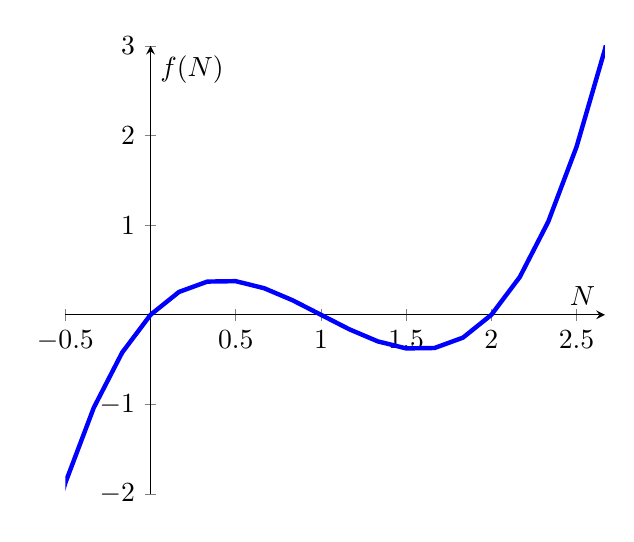
\begin{tikzpicture}[scale=1.0]
\begin{axis}[
        axis x line=middle,
        axis y line=middle,
        ymax=3, ymin=-2, ylabel=$f(N)$,
        xlabel=$N$
        ]
    \addplot[domain=-1:3, blue, ultra thick] {x * (x - 2) * (x - 1)};
\end{axis}
\end{tikzpicture}
\caption{$y = N(N - \a)(N - \b)$}
\end{figure}

Then we consider the small perturbations around the steady states and it was a linear ODE that resulted in exponential decay or just an exponential. We don't need to do this though, as we can look at the phase space as it has split up the graph into regions. These regions are $(-\infty, 0],\, [0, \a],\, [\a, \b]$.

\begin{itemize}
  \item For $(-\infty, 0]$ the system declines and so we draw arrows going away from $0$ to the left.
  \item Then it's going to move towards $\a$ from $0$ where it stops at the steady state $\a$.
  \item From $\a$ to $\b$, the particle is going to move from $\b$ to $\a$.
  \item Anything larger than $\b$, it shoots off to infinity.
\end{itemize}

From this, we can talk about the stability of the stable states. We can call $0$ and $\b$ unstable and we can say $\a$ is a stable fixed point. So now we ask how do we describe $N(t)$ from this information?

\begin{figure}[!ht]
\centering
\begin{tikzpicture}[scale=1.0]
\begin{axis}[
        axis x line=middle,
        axis y line=middle,
        ymax=3, ymin=0, ylabel=$f(N)$,
        xlabel=$N$
        ]
    \addplot[domain=0:3, blue, dotted, ultra thick] {1};
    \addplot[domain=0:3, blue, dotted, ultra thick] {2};
\end{axis}
\end{tikzpicture}
\caption{Steady States of the system}
\end{figure}

\section{Modelling Spruce Budworm}
Spruce Budworm eats spruce trees and populations have been watched and there exists some oscillatory behavior. Let's formulate some sort of model, firstly with a cartoon and then the assumptions to create a mathematical model. We consider $N = \text{ population density} \in \R$. We assume that;
\begin{itemize}
  \item bounded growth, the logistic growth model (e.g. limited resources)
  \item predation (by birds)
\end{itemize}
and so we can write,
$$ \di N t = rN\left(1 - \frac{N}{k} \right) - p(N)$$
and now a few assumptions for $p$,
\begin{itemize}
  \item no predation if no prey, $p(0) = 0$
  \item predator population is not infinite, this means the rate of predation saturates as $n \to \infty$.
  \item If $n$ is small, $p(N)$ is small.
\end{itemize}
We want a sigmoidal form of function so we can encode these assumptions.

\begin{figure}[!ht]
\centering
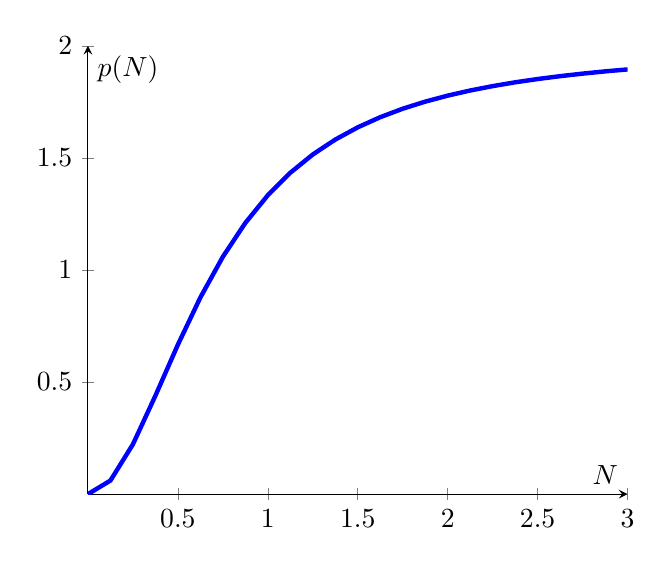
\begin{tikzpicture}[scale=1.0]
\begin{axis}[
        axis x line=middle,
        axis y line=middle,
        ymax=2, ymin=0, ylabel=$p(N)$,
        xlabel=$N$
        ]
    \addplot[domain=0:3, blue, ultra thick] {2*x*x / (1/2 + x*x)};
\end{axis}
\end{tikzpicture}
\caption{Sigmoidal Function, $p(N)$}
\end{figure}

We will let $p(N) = \frac{BN^2}{A^2 + N^2}$, which will work quite nicely. This is a function seen all over Maths Biology. Hence, we write,
$$ \di N t = r_B N \left( 1- \frac{N}{k_B} \right) - \frac{BN^2}{A^2 + N^2} $$
where $r_B, k_B, B, A > 0$ and $N \ge 0$.
In mathematical Biology we don't really have any big ideas about what our parameters are, we talk more generally about what our parameters actually mean. This makes it harder to know what's going on with multiple parameters.

\subsection{Scaling and Non-dimensionalisation}
The goal is to scale variables and time such that we get an equivalent system with fewer parameters, equivalent is in relation to the steady states and their stabilities.\\

Our stategy is to find constants $\a$ and $\b$ so that $u = \a$ and $\tau = \b t$ yields a simpler system. The first thing we do is write down a new system, $\di u \tau$.
$$ \di u \tau = \di N t \di t \tau \di u N $$
and so we can do some algebra (ommited), then we get to a point where we want to choose some values for our placeholders of $\a$ and $\b$, given the form of the system, we choose that $\a = \frac{1}{A}$ and $\b = B\a = \frac{B}{A}$ and hence the system simplifies to,
$$ \d u {\tau} = ru (1 - \frac{u}{q}) + \frac{u^2}{1 + u^2} $$
